\section{Demo sản phẩm}

\subsection{Video Demo hệ thống (8--10 phút)}
\begin{itemize}
    \item \textbf{Link video demo công khai:} \textit{\_TODO: Dán link YouTube hoặc Google Drive công khai tại đây\_}
    \item \textbf{Kịch bản quay chi tiết:} Thực hiện theo 8 phần trong tệp \texttt{docs/DEMO\_SCRIPT.md} (luồng Sinh viên, luồng Operator, đổi Sáng/Tối \& VN/EN, và 3 demo bắt buộc).
\end{itemize}

\subsection{Hình ảnh minh họa theo từng Use Case (UC1 -- UC17)}
Dưới đây là chuỗi ảnh chụp màn hình chạy thực tế trên ứng dụng web \textbf{E-Hub} cho toàn bộ 17 Use Case thuộc hai phân hệ Sinh viên và Đơn vị vận hành (Operator).

\subsubsection{Phân hệ Sinh viên và Dùng chung}

\paragraph{UC1 --- Tìm phương tiện và Hub phù hợp:}
Sinh viên truy cập \texttt{/student/search}, xem bản đồ 5 Hub khu vực ĐHQG-HCM, vị trí hiện tại (BK CS2) và tuyến đường đi bộ tới trạm được chọn.
\begin{figure}[H]
    \centering
    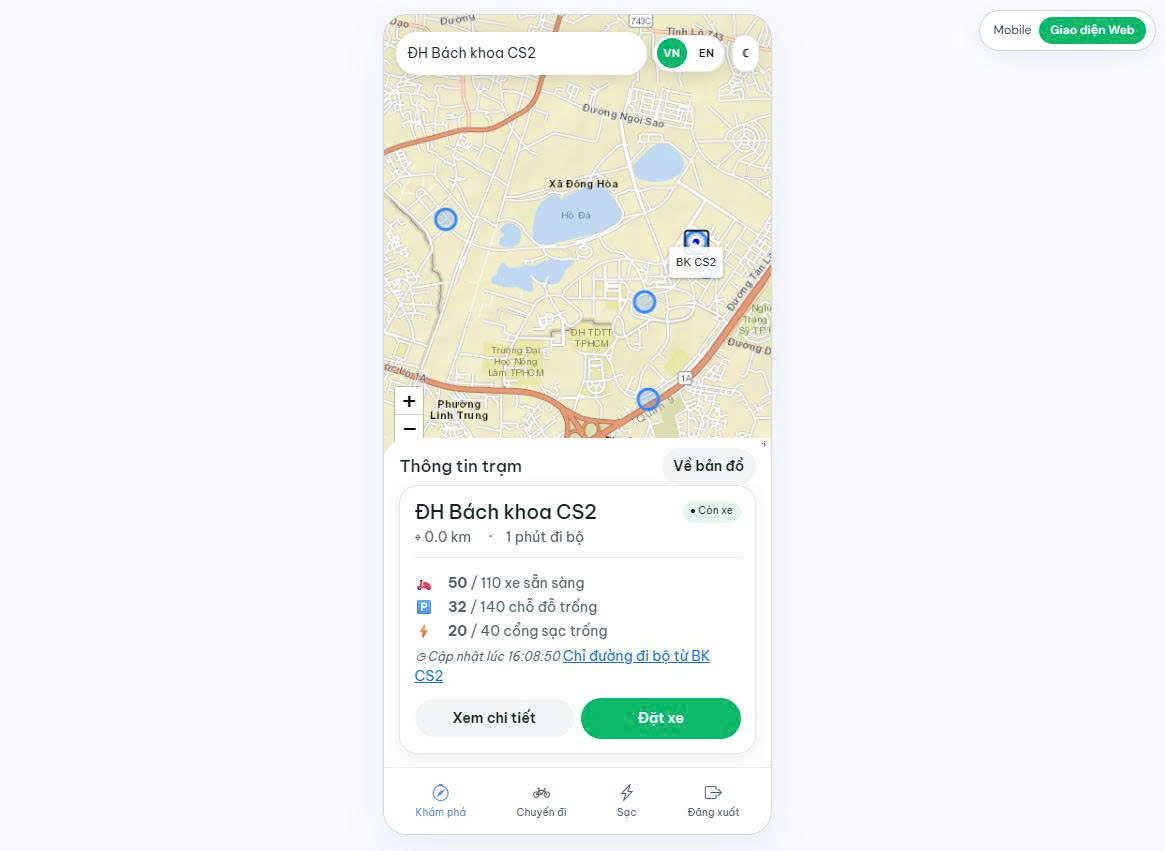
\includegraphics[width=0.88\textwidth]{demo_UC1-17/UC01_tim_phuong_tien_va_hub.jpg}
    \caption{UC1 --- Giao diện tìm kiếm phương tiện và bản đồ điều hướng tại Hub (\texttt{/student/search})}
    \label{fig:demo_uc01}
\end{figure}

\paragraph{UC2 --- Xem trạng thái phương tiện và Hub:}
Xem chi tiết số xe sẵn sàng, chỗ đỗ trống, cổng sạc và danh sách từng xe tại Hub kèm mức pin (\texttt{/student/resource}).
\begin{figure}[H]
    \centering
    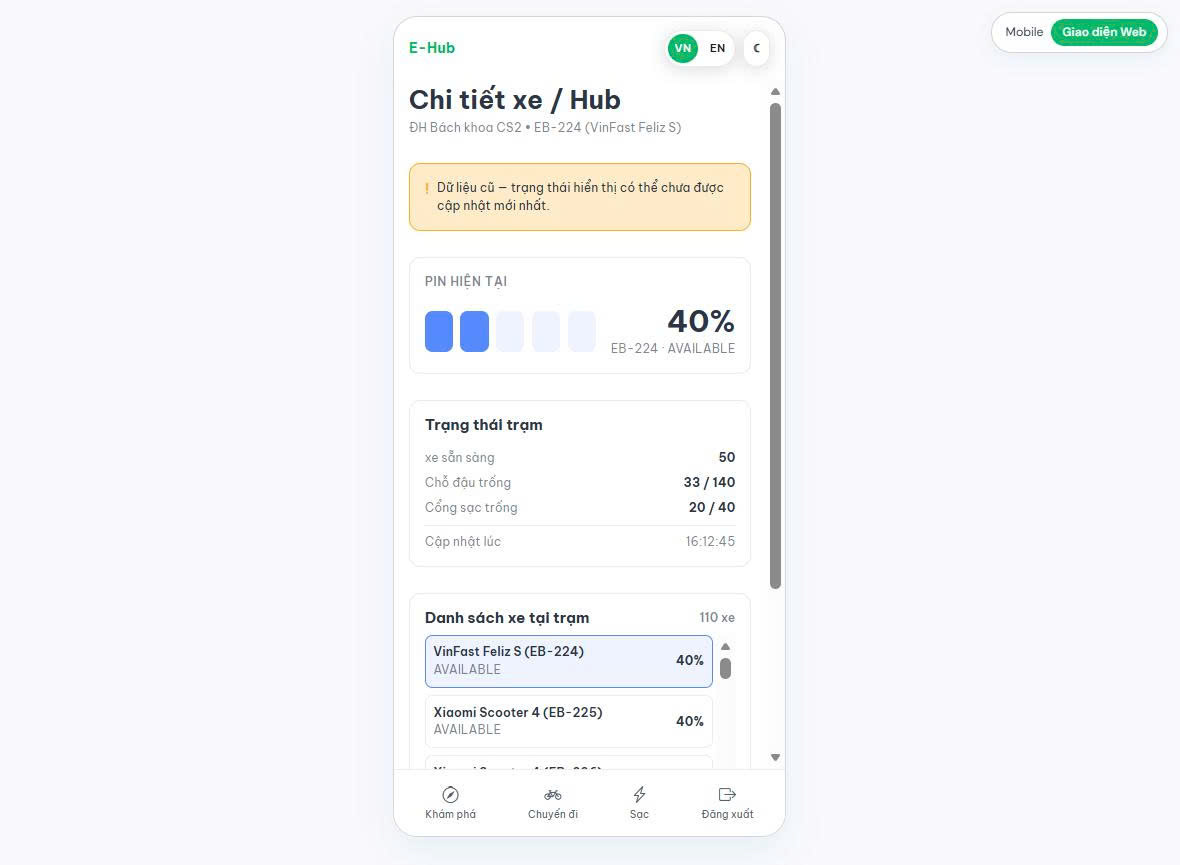
\includegraphics[width=0.88\textwidth]{demo_UC1-17/UC02_xem_trang_thai_phuong_tien_va_hub.jpg}
    \caption{UC2 --- Màn hình chi tiết trạng thái phương tiện và Hub (\texttt{/student/resource})}
    \label{fig:demo_uc02}
\end{figure}

\paragraph{UC3 --- Đặt xe:}
Sinh viên chọn phương tiện cụ thể trên modal đặt xe và nhận thông báo giữ xe thành công kèm mã đặt chỗ.
\begin{figure}[H]
    \centering
    \begin{subfigure}[b]{0.48\textwidth}
        \centering
        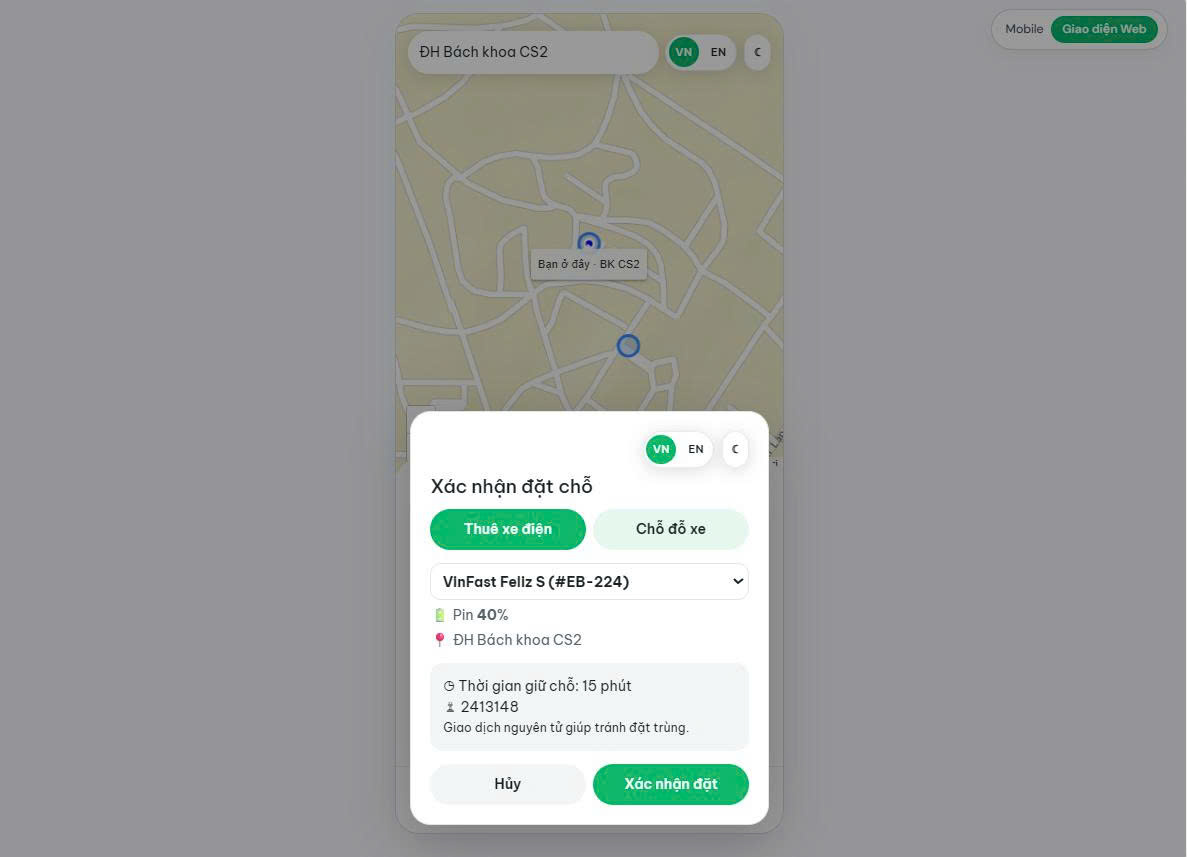
\includegraphics[width=\textwidth]{demo_UC1-17/UC03_dat_xe_1_form.jpg}
        \caption{Chọn xe và xác nhận thông tin đặt xe}
    \end{subfigure}
    \hfill
    \begin{subfigure}[b]{0.48\textwidth}
        \centering
        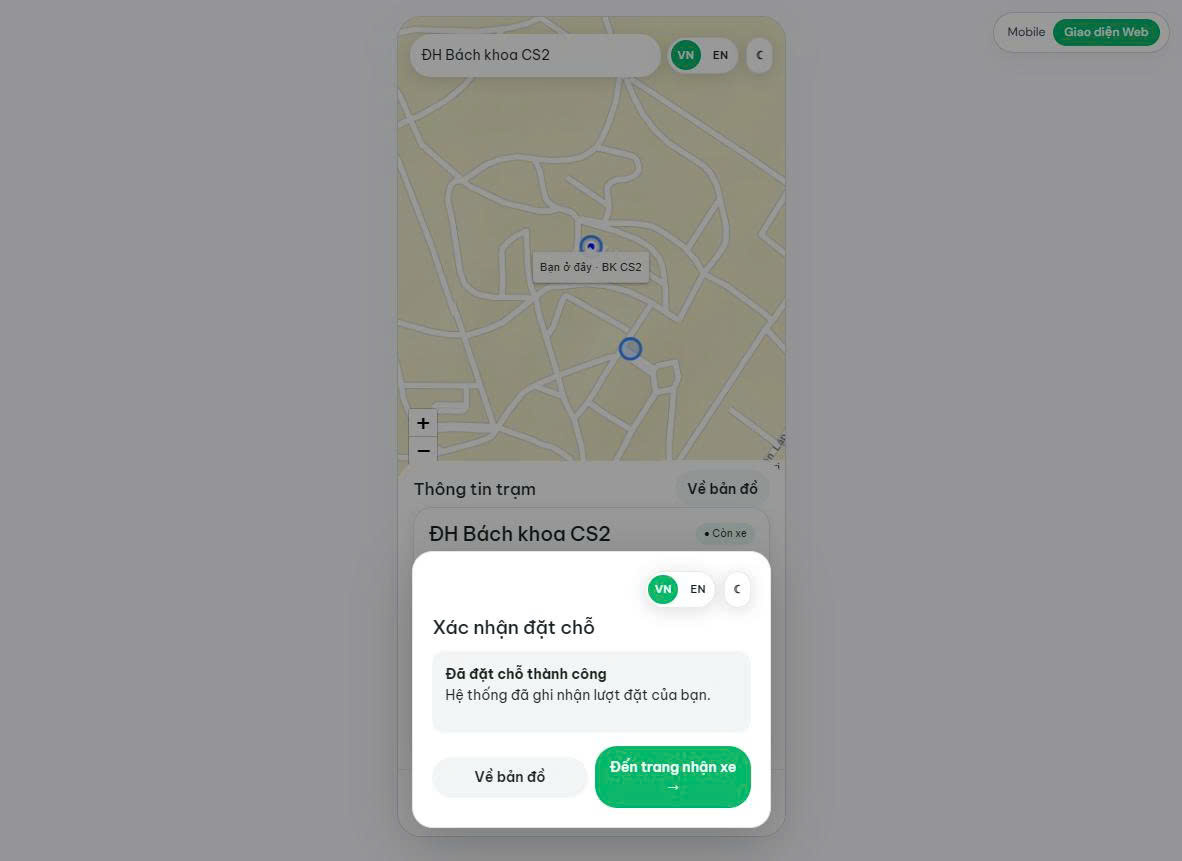
\includegraphics[width=\textwidth]{demo_UC1-17/UC03_dat_xe_2_thanh_cong.jpg}
        \caption{Đặt xe thành công và điều hướng nhận xe}
    \end{subfigure}
    \caption{UC3 --- Luồng đặt phương tiện trên cổng Sinh viên}
    \label{fig:demo_uc03}
\end{figure}

\paragraph{UC4 --- Đặt chỗ đỗ xe:}
Chức năng đặt trước chỗ đỗ theo khung giờ, kiểm tra chặn thời gian quá khứ và xác nhận đặt chỗ thành công.
\begin{figure}[H]
    \centering
    \begin{subfigure}[b]{0.48\textwidth}
        \centering
        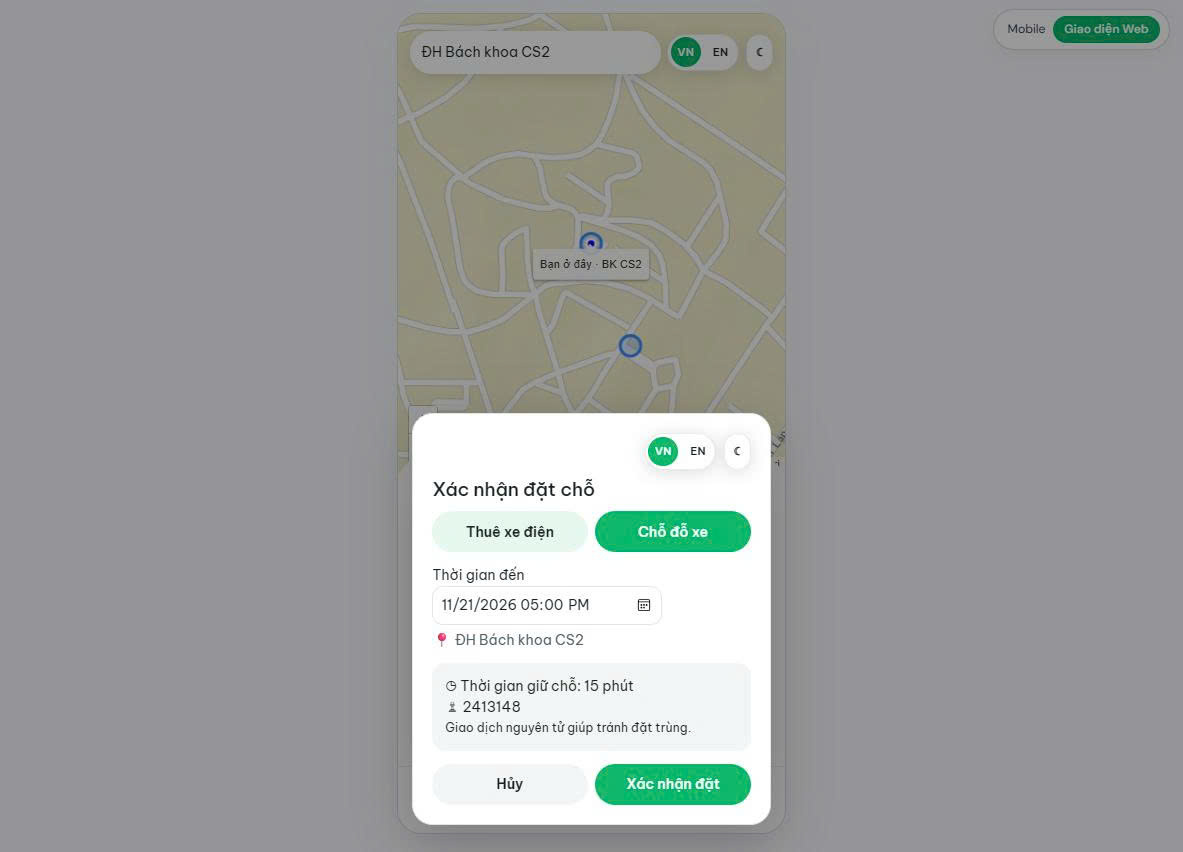
\includegraphics[width=\textwidth]{demo_UC1-17/UC04_dat_cho_do_xe_1_form.jpg}
        \caption{Chọn khung giờ đặt chỗ đỗ xe}
    \end{subfigure}
    \hfill
    \begin{subfigure}[b]{0.48\textwidth}
        \centering
        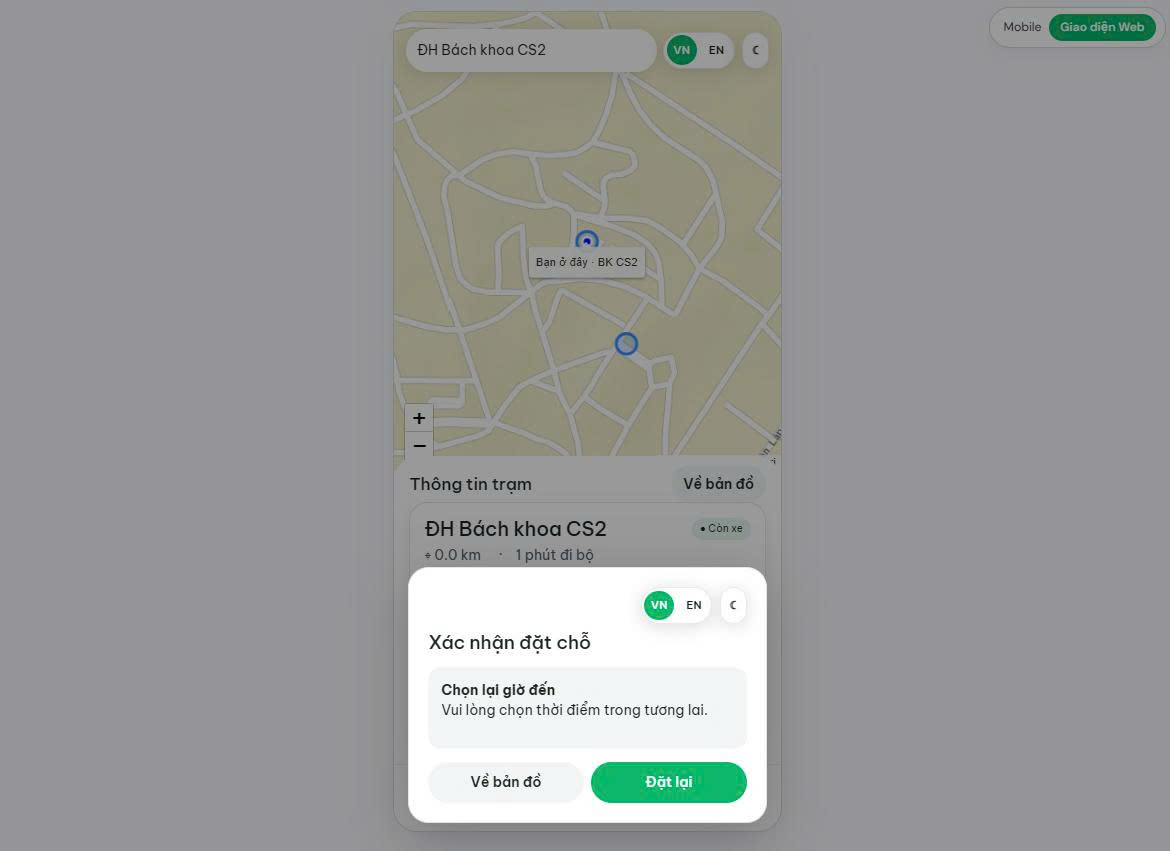
\includegraphics[width=\textwidth]{demo_UC1-17/UC04_dat_cho_do_xe_2_chan_gio_qua_khu.jpg}
        \caption{Ràng buộc chặn chọn giờ trong quá khứ}
    \end{subfigure}

    \vspace{0.3cm}
    \begin{subfigure}[b]{0.58\textwidth}
        \centering
        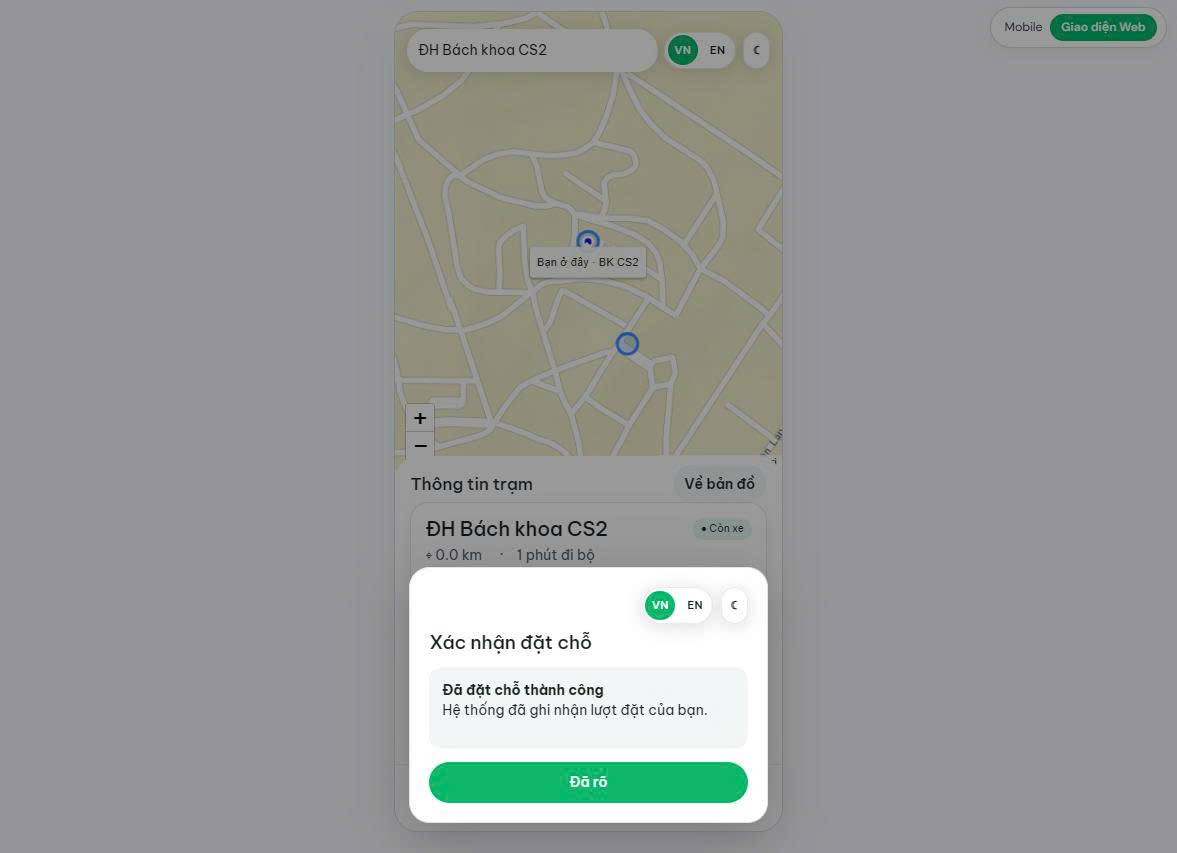
\includegraphics[width=\textwidth]{demo_UC1-17/UC04_dat_cho_do_xe_3_thanh_cong.jpg}
        \caption{Xác nhận đặt chỗ đỗ xe thành công}
    \end{subfigure}
    \caption{UC4 --- Luồng đặt chỗ đỗ xe và kiểm tra ràng buộc thời gian}
    \label{fig:demo_uc04}
\end{figure}

\paragraph{UC5 --- Nhận phương tiện:}
Sinh viên xác nhận nhận xe đã đặt tại trạm (\texttt{/student/pickup}) để chuyển trạng thái sang chuyến đi đang hoạt động (\texttt{/student/ride}).
\begin{figure}[H]
    \centering
    \begin{subfigure}[b]{0.48\textwidth}
        \centering
        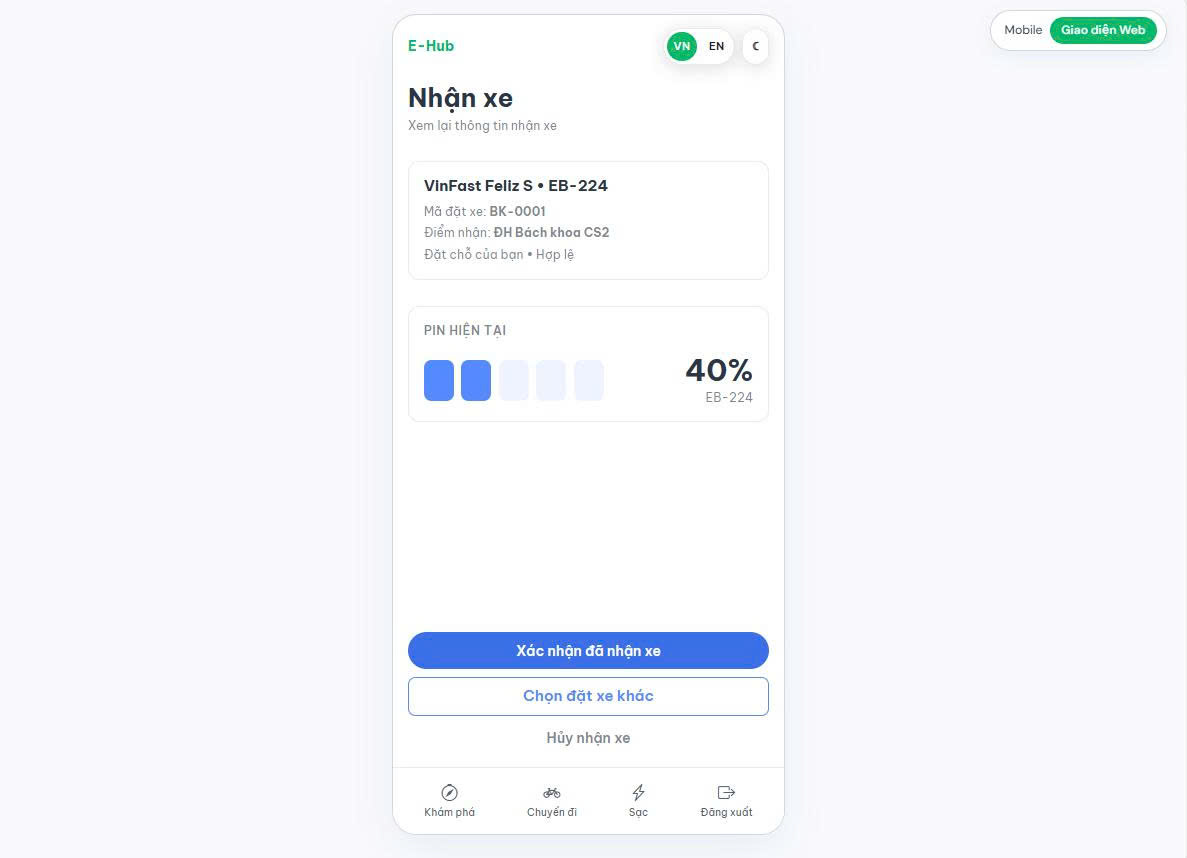
\includegraphics[width=\textwidth]{demo_UC1-17/UC05_nhan_phuong_tien_1_xac_nhan.jpg}
        \caption{Xác nhận thông tin trước khi nhận xe}
    \end{subfigure}
    \hfill
    \begin{subfigure}[b]{0.48\textwidth}
        \centering
        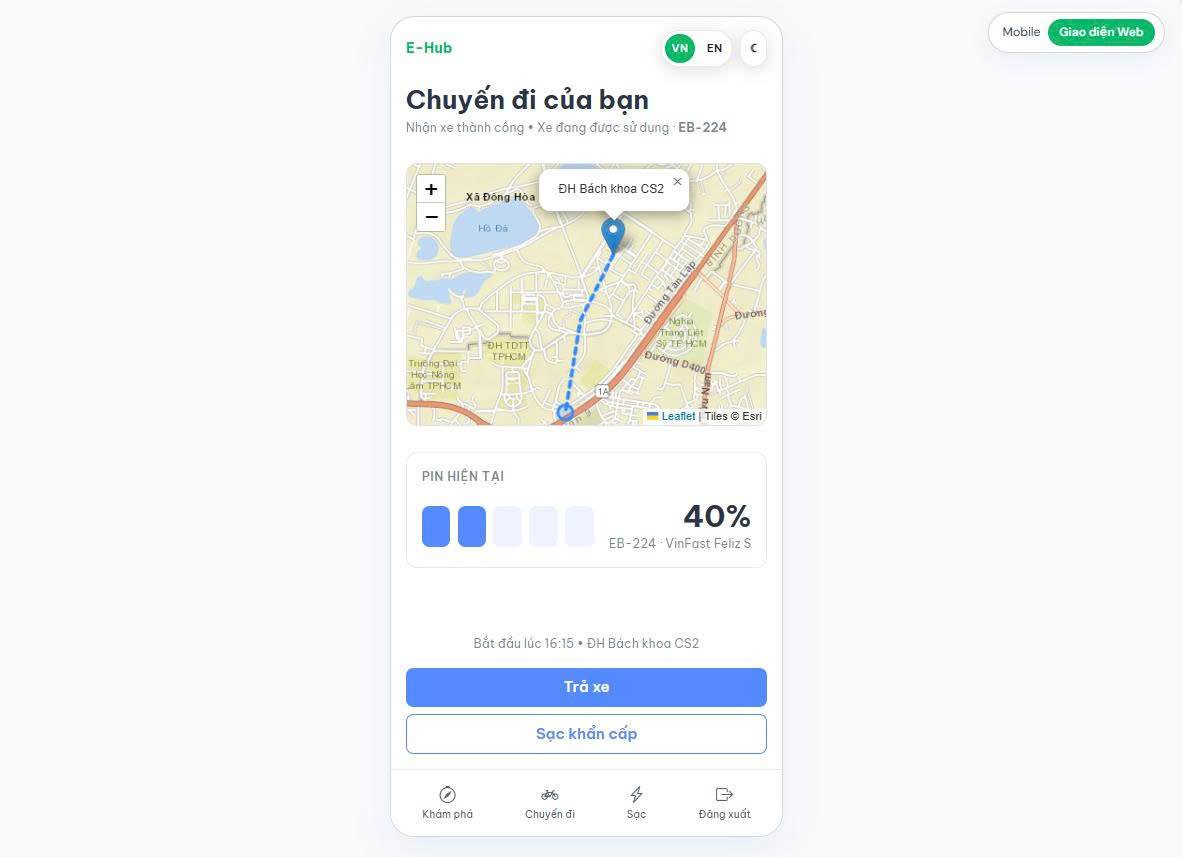
\includegraphics[width=\textwidth]{demo_UC1-17/UC05_nhan_phuong_tien_2_chuyen_di.jpg}
        \caption{Chuyến đi bắt đầu kèm bản đồ và mức pin}
    \end{subfigure}
    \caption{UC5 --- Xác nhận nhận phương tiện và theo dõi chuyến đi}
    \label{fig:demo_uc05}
\end{figure}

\paragraph{UC6 --- Trả phương tiện:}
Chọn trạm trả xe còn chỗ trống (\texttt{/student/return}) và hoàn tất giao dịch trả xe (\texttt{/student/returned}).
\begin{figure}[H]
    \centering
    \begin{subfigure}[b]{0.48\textwidth}
        \centering
        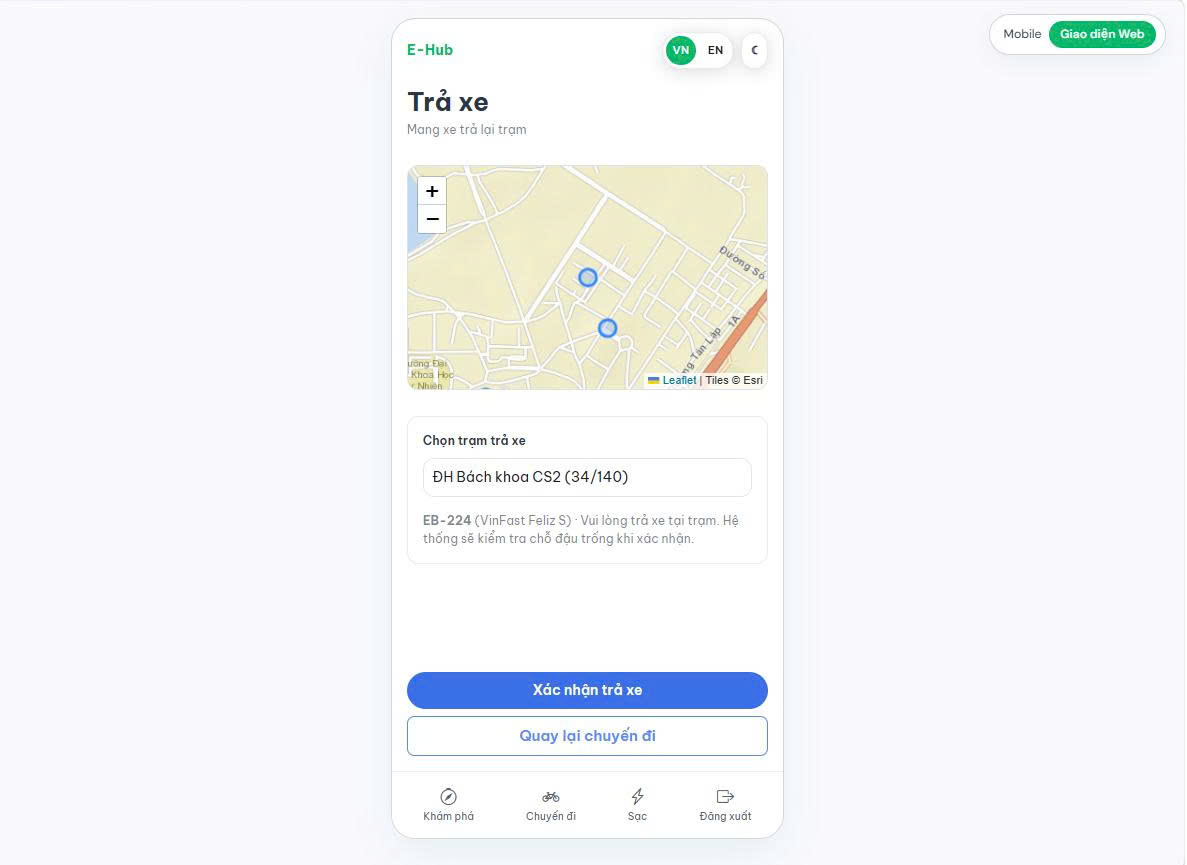
\includegraphics[width=\textwidth]{demo_UC1-17/UC06_tra_phuong_tien_1_form.jpg}
        \caption{Chọn trạm trả xe trên giao diện trả xe}
    \end{subfigure}
    \hfill
    \begin{subfigure}[b]{0.48\textwidth}
        \centering
        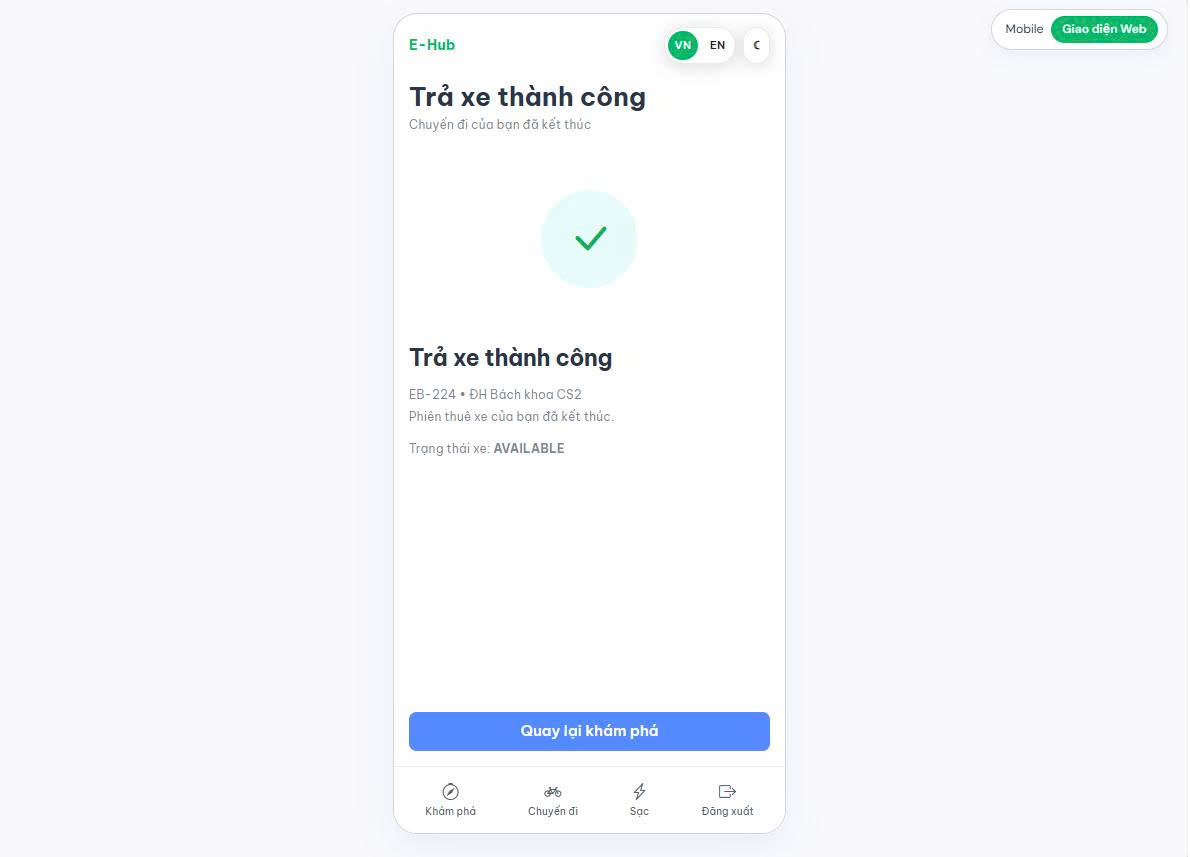
\includegraphics[width=\textwidth]{demo_UC1-17/UC06_tra_phuong_tien_2_thanh_cong.jpg}
        \caption{Thông báo trả phương tiện thành công}
    \end{subfigure}
    \caption{UC6 --- Luồng trả phương tiện tại Hub}
    \label{fig:demo_uc06}
\end{figure}

\paragraph{UC7 --- Đăng ký sạc:}
Hỗ trợ gợi ý trạm sạc khẩn cấp gần nhất, chọn khung giờ sạc khả dụng, xem lại thông tin và hoàn tất đăng ký cổng sạc.
\begin{figure}[H]
    \centering
    \begin{subfigure}[b]{0.46\textwidth}
        \centering
        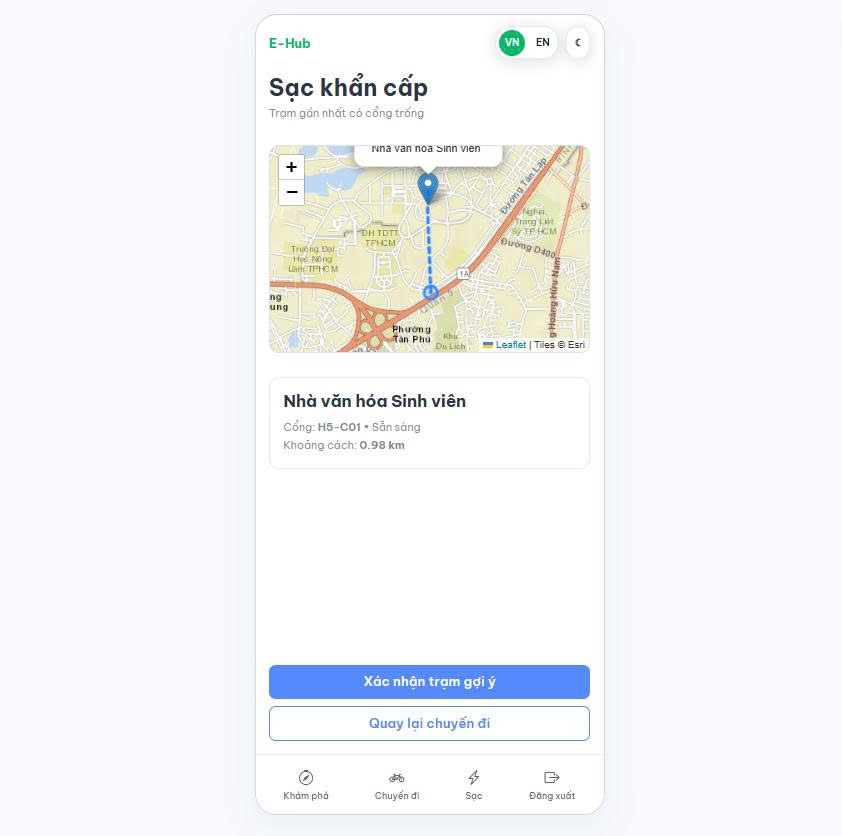
\includegraphics[width=\textwidth]{demo_UC1-17/UC07_dang_ky_sac_1_sac_khan_cap.jpg}
        \caption{Gợi ý trạm sạc khẩn cấp gần nhất}
    \end{subfigure}
    \hfill
    \begin{subfigure}[b]{0.46\textwidth}
        \centering
        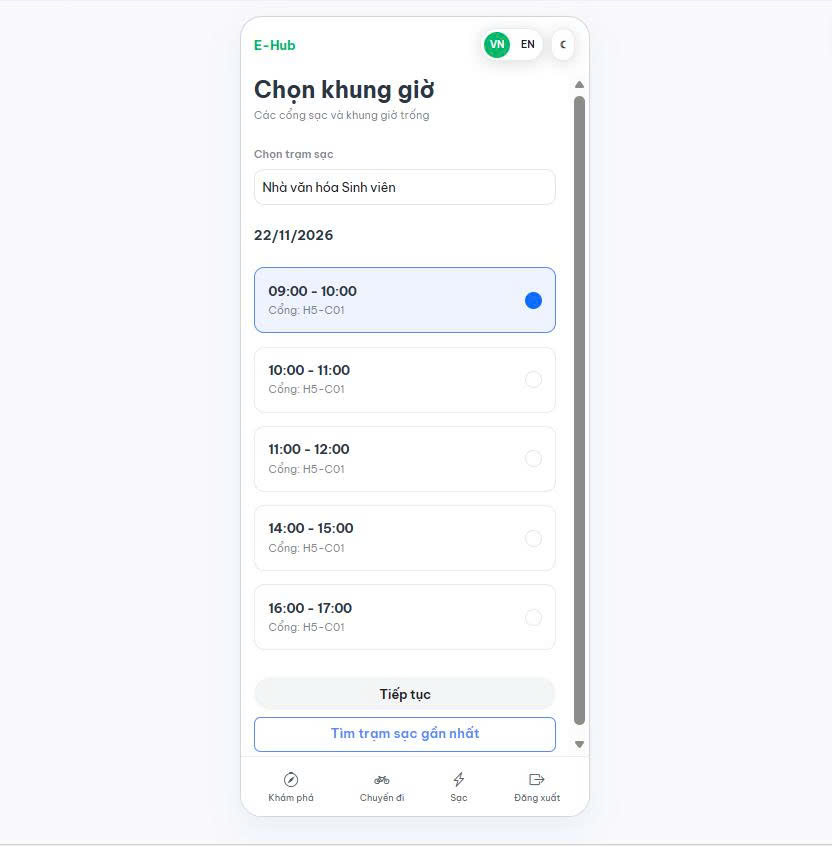
\includegraphics[width=\textwidth]{demo_UC1-17/UC07_dang_ky_sac_2_chon_gio.jpg}
        \caption{Chọn Hub và khung giờ sạc}
    \end{subfigure}

    \vspace{0.3cm}
    \begin{subfigure}[b]{0.46\textwidth}
        \centering
        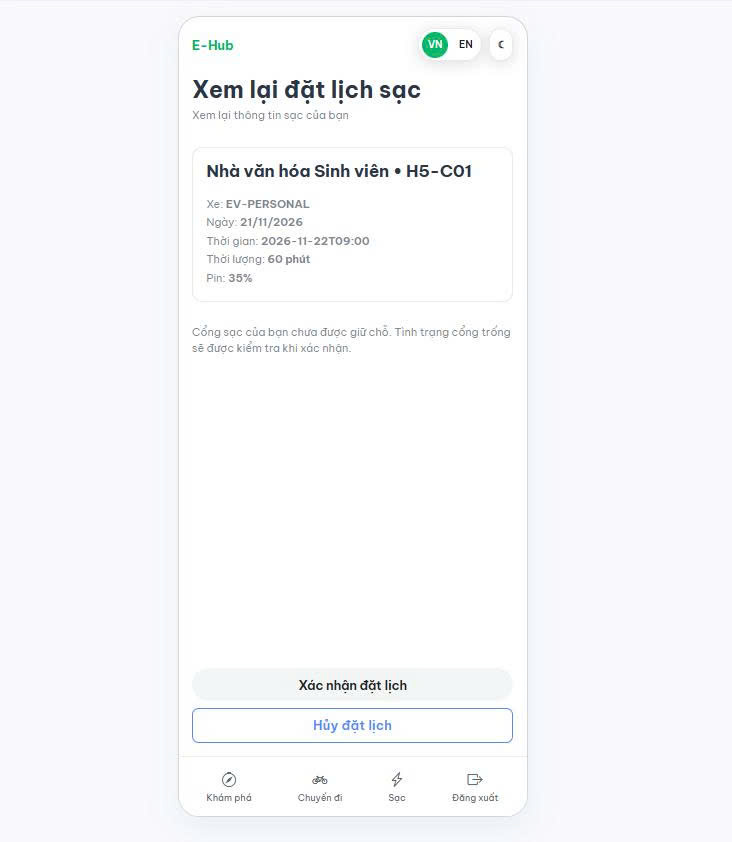
\includegraphics[width=\textwidth]{demo_UC1-17/UC07_dang_ky_sac_3_xem_lai.jpg}
        \caption{Xem lại thông tin trước khi xác nhận}
    \end{subfigure}
    \hfill
    \begin{subfigure}[b]{0.46\textwidth}
        \centering
        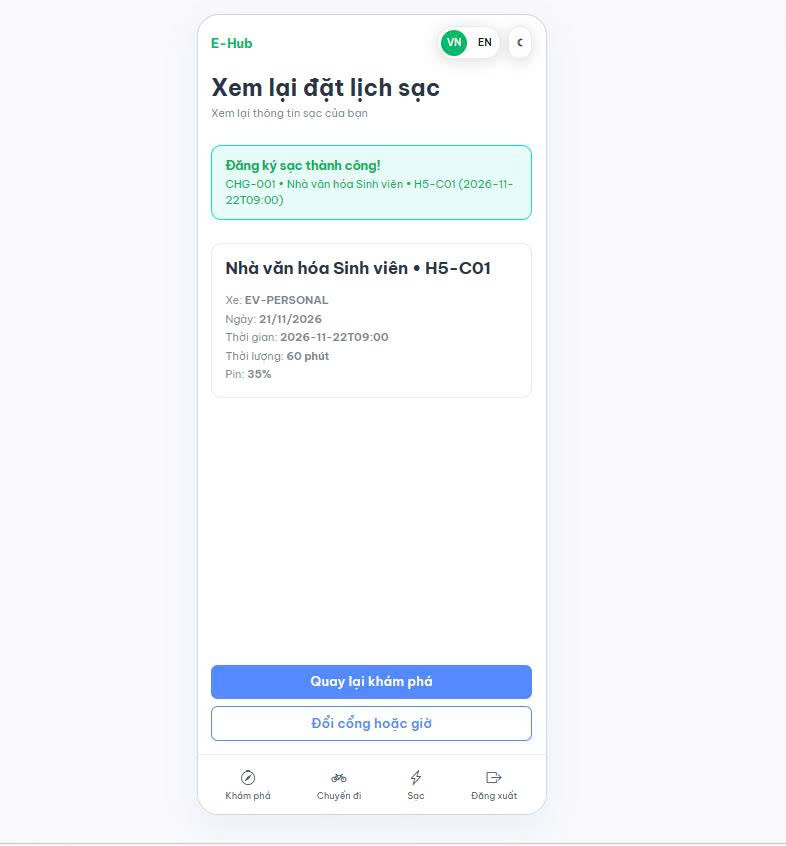
\includegraphics[width=\textwidth]{demo_UC1-17/UC07_dang_ky_sac_4_thanh_cong.jpg}
        \caption{Đăng ký khung giờ sạc thành công}
    \end{subfigure}
    \caption{UC7 --- Chuỗi màn hình gợi ý sạc khẩn cấp và đăng ký lịch sạc}
    \label{fig:demo_uc07}
\end{figure}

\paragraph{UC15 --- Tùy chỉnh giao diện:}
Chuyển đổi trực tiếp giữa chế độ Sáng/Tối (Light/Dark Mode) và song ngữ Việt/Anh (VN/EN) mà không tải lại trang.
\begin{figure}[H]
    \centering
    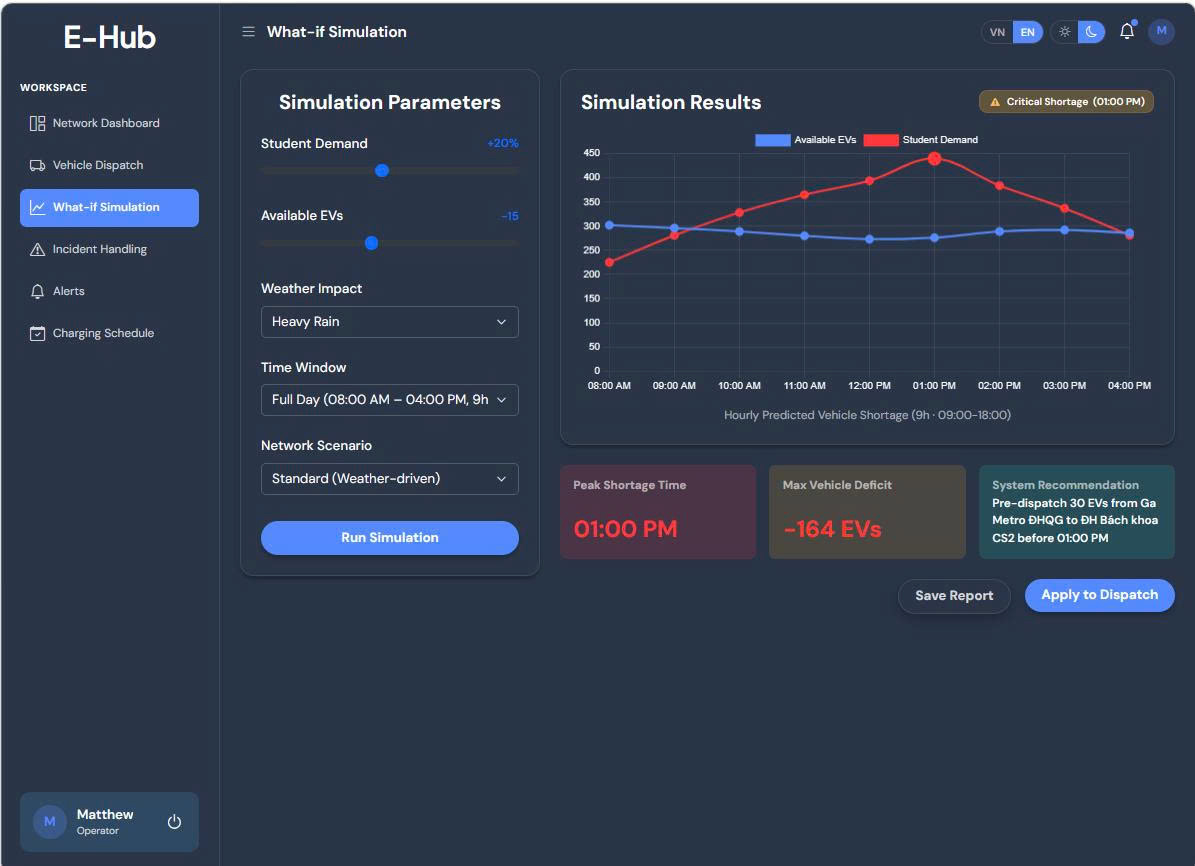
\includegraphics[width=0.88\textwidth]{demo_UC1-17/UC15_tuy_chinh_giao_dien_dark_en.jpg}
    \caption{UC15 --- Giao diện hệ thống ở chế độ Nền tối (Dark Mode) và Tiếng Anh (EN)}
    \label{fig:demo_uc15}
\end{figure}

\paragraph{UC17 --- Xác thực SSO Dual-Portal:}
Tách biệt hoàn toàn cổng đăng nhập cho Sinh viên (\texttt{/login}) và Đơn vị vận hành (\texttt{/operator/login}), kiểm tra phân quyền theo vai trò tài khoản.
\begin{figure}[H]
    \centering
    \begin{subfigure}[b]{0.48\textwidth}
        \centering
        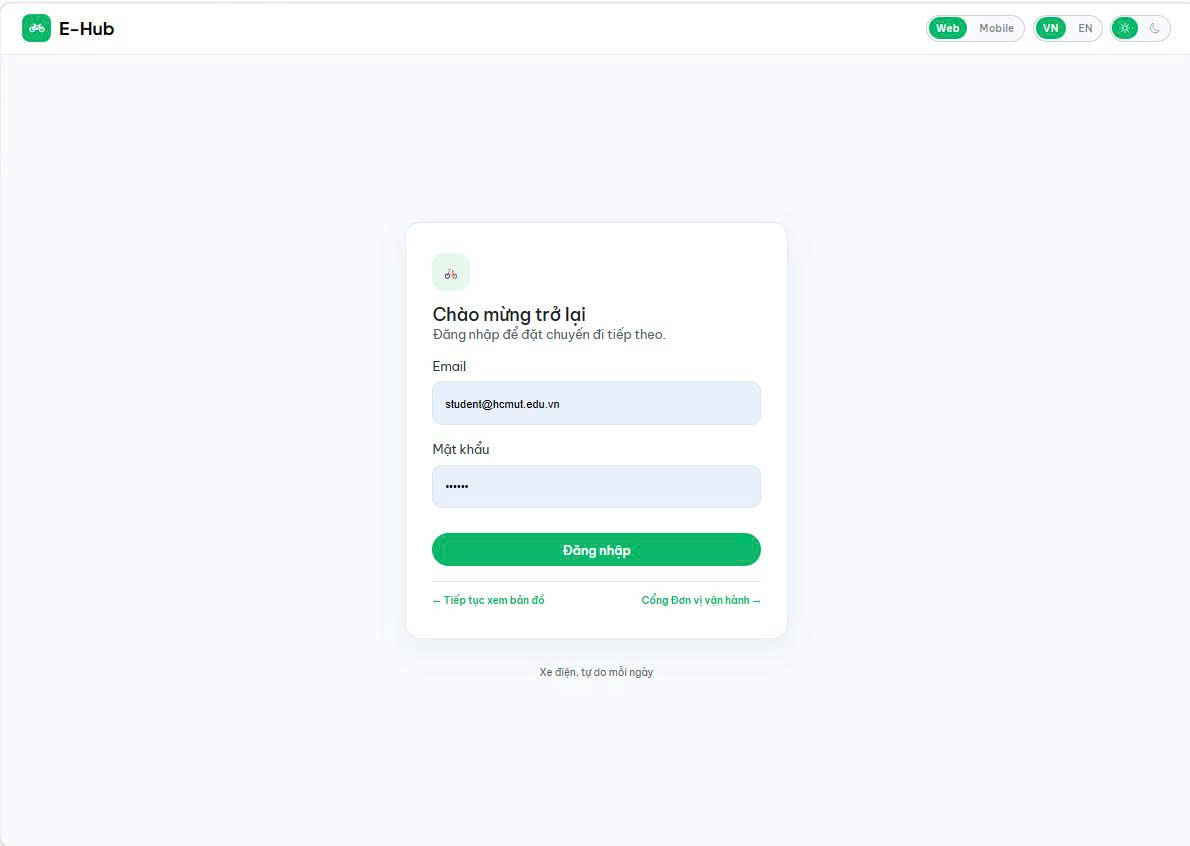
\includegraphics[width=\textwidth]{demo_UC1-17/UC17_xac_thuc_sso_1_student.jpg}
        \caption{Cổng đăng nhập SSO dành cho Sinh viên}
    \end{subfigure}
    \hfill
    \begin{subfigure}[b]{0.48\textwidth}
        \centering
        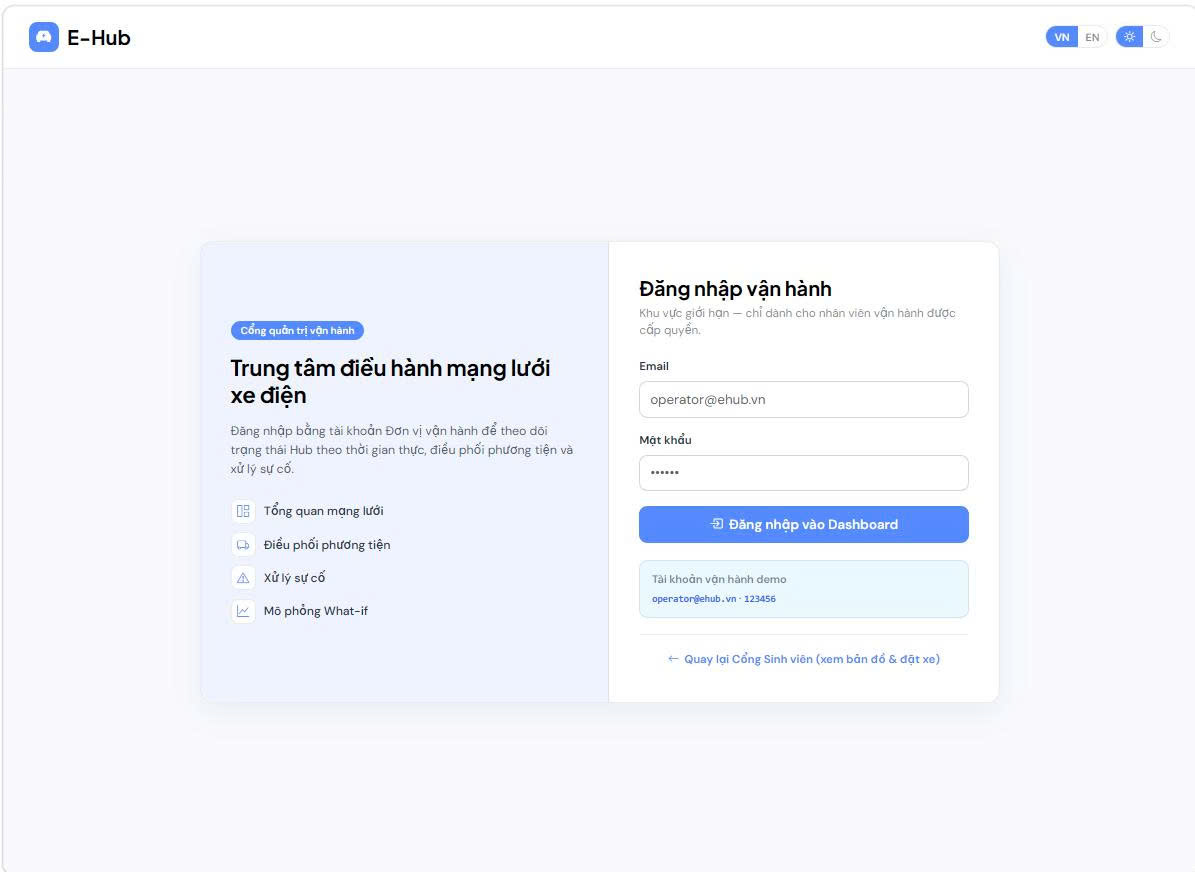
\includegraphics[width=\textwidth]{demo_UC1-17/UC17_xac_thuc_sso_2_operator.jpg}
        \caption{Cổng đăng nhập riêng cho Operator}
    \end{subfigure}
    \caption{UC17 --- Xác thực SSO tách biệt hai phân hệ (Dual-Portal Login)}
    \label{fig:demo_uc17}
\end{figure}

\subsubsection{Phân hệ Đơn vị vận hành (Operator)}

\paragraph{UC8 --- Giám sát mạng lưới Hub:}
Trang tổng quan Dashboard (\texttt{/operator/overview}) hiển thị các chỉ số KPI toàn mạng, bảng tải 5 Hub cập nhật thời gian thực và cảnh báo nổi bật.
\begin{figure}[H]
    \centering
    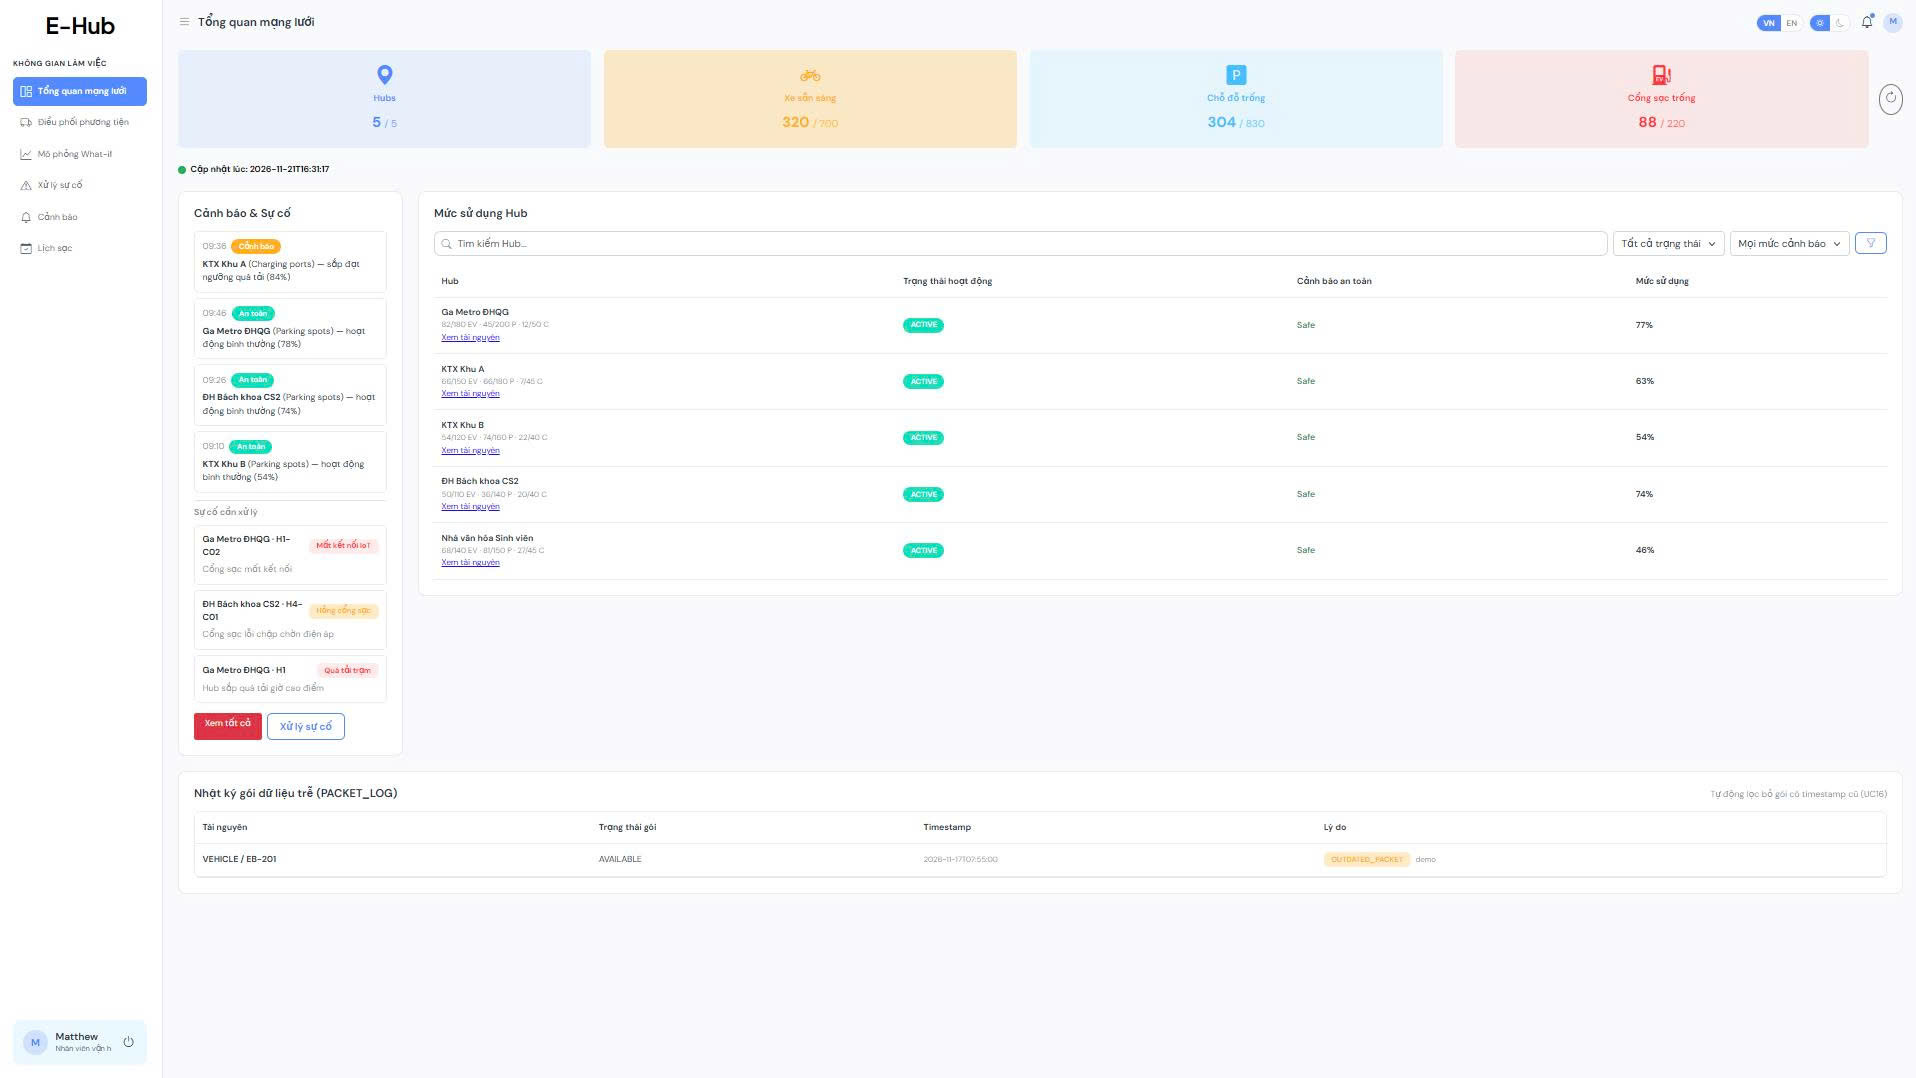
\includegraphics[width=0.92\textwidth]{demo_UC1-17/UC08_giam_sat_mang_luoi_hub.jpg}
    \caption{UC8 --- Bảng điều khiển tổng quan mạng lưới Hub (\texttt{/operator/overview})}
    \label{fig:demo_uc08}
\end{figure}

\paragraph{UC9 --- Theo dõi tài nguyên Hub:}
Quản lý tập trung trạng thái của 700 phương tiện, 830 chỗ đỗ và 220 cổng sạc kèm thanh tìm kiếm và bộ lọc theo Hub (\texttt{/operator/resources}).
\begin{figure}[H]
    \centering
    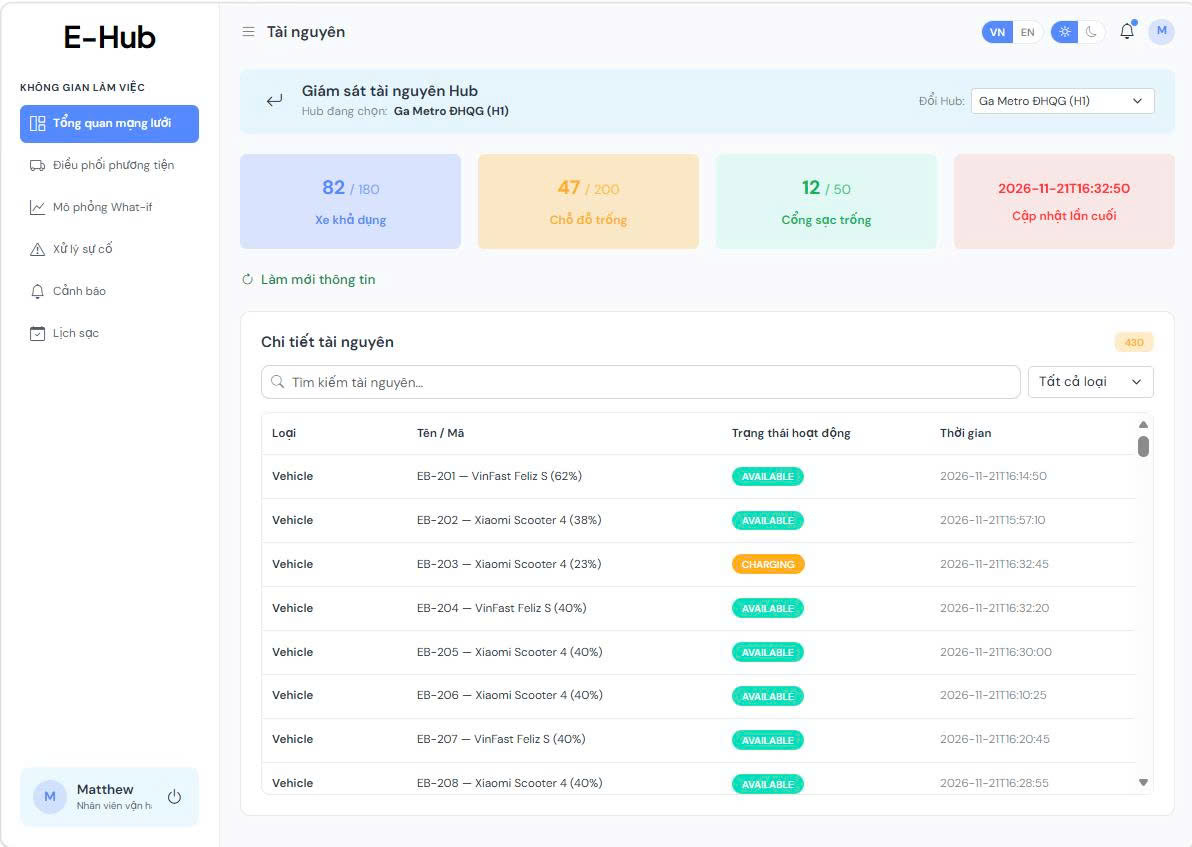
\includegraphics[width=0.88\textwidth]{demo_UC1-17/UC09_theo_doi_tai_nguyen.jpg}
    \caption{UC9 --- Màn hình theo dõi tài nguyên từng Hub (\texttt{/operator/resources})}
    \label{fig:demo_uc09}
\end{figure}

\paragraph{UC10 --- Cảnh báo quá tải:}
Hiển thị danh sách cảnh báo quá tải phân loại theo 3 mức độ nghiêm trọng (\texttt{HIGH}, \texttt{MEDIUM}, \texttt{LOW}) để vận hành ưu tiên xử lý (\texttt{/operator/alerts}).
\begin{figure}[H]
    \centering
    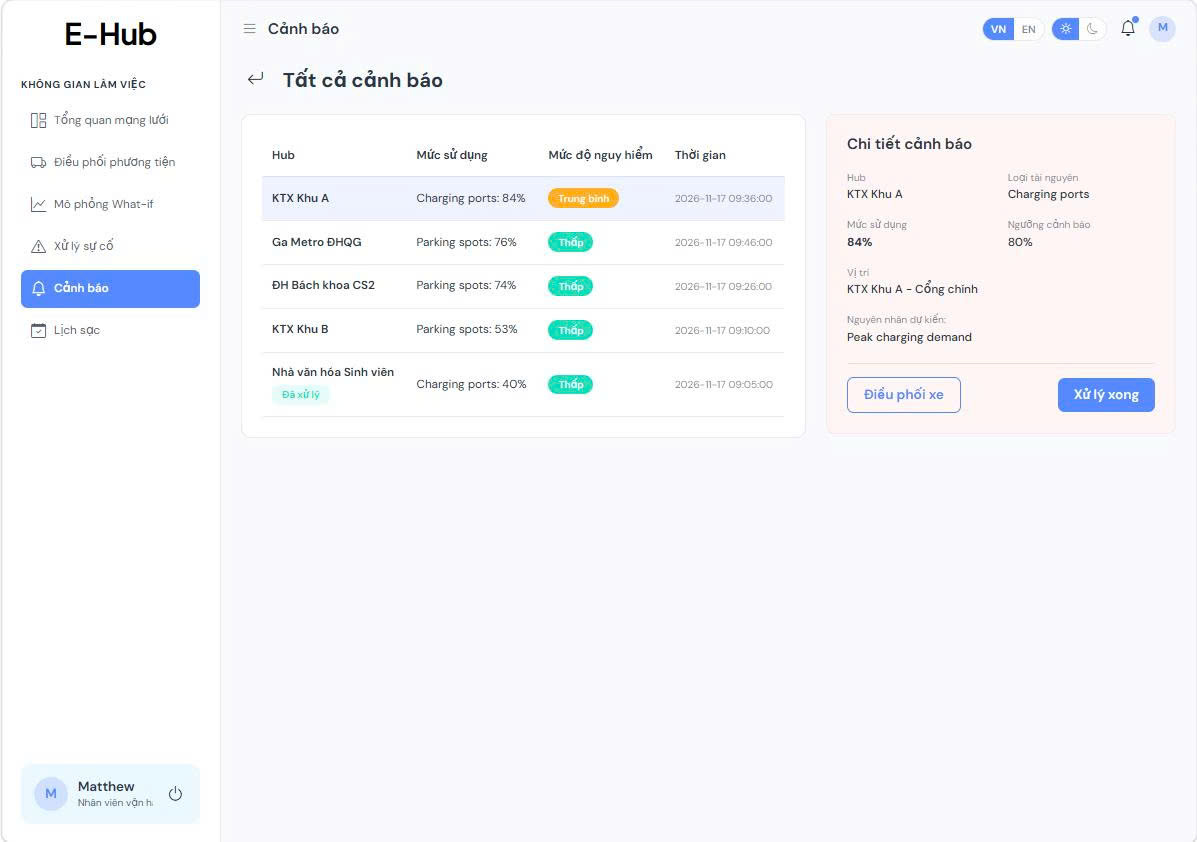
\includegraphics[width=0.88\textwidth]{demo_UC1-17/UC10_xem_canh_bao_qua_tai.jpg}
    \caption{UC10 --- Màn hình cảnh báo quá tải tại các Hub (\texttt{/operator/alerts})}
    \label{fig:demo_uc10}
\end{figure}

\paragraph{UC11 --- Điều phối phương tiện:}
Operator chọn Hub nguồn/đích trực tiếp trên bản đồ Leaflet (\texttt{/operator/dispatch}), chọn các xe cần chuyển và tạo lệnh điều phối.
\begin{figure}[H]
    \centering
    \begin{subfigure}[b]{0.48\textwidth}
        \centering
        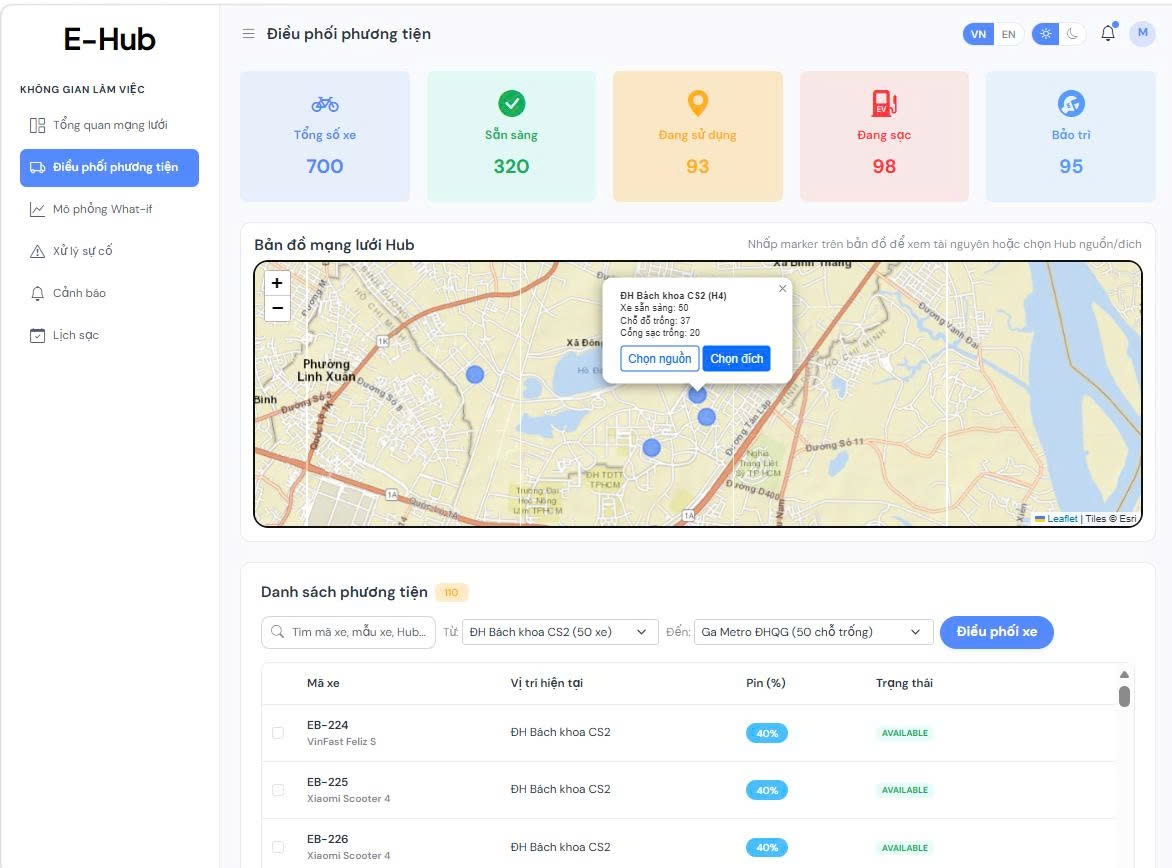
\includegraphics[width=\textwidth]{demo_UC1-17/UC11_dieu_phoi_phuong_tien_1_chon_hub.jpg}
        \caption{Chọn Hub nguồn và đích trên bản đồ}
    \end{subfigure}
    \hfill
    \begin{subfigure}[b]{0.48\textwidth}
        \centering
        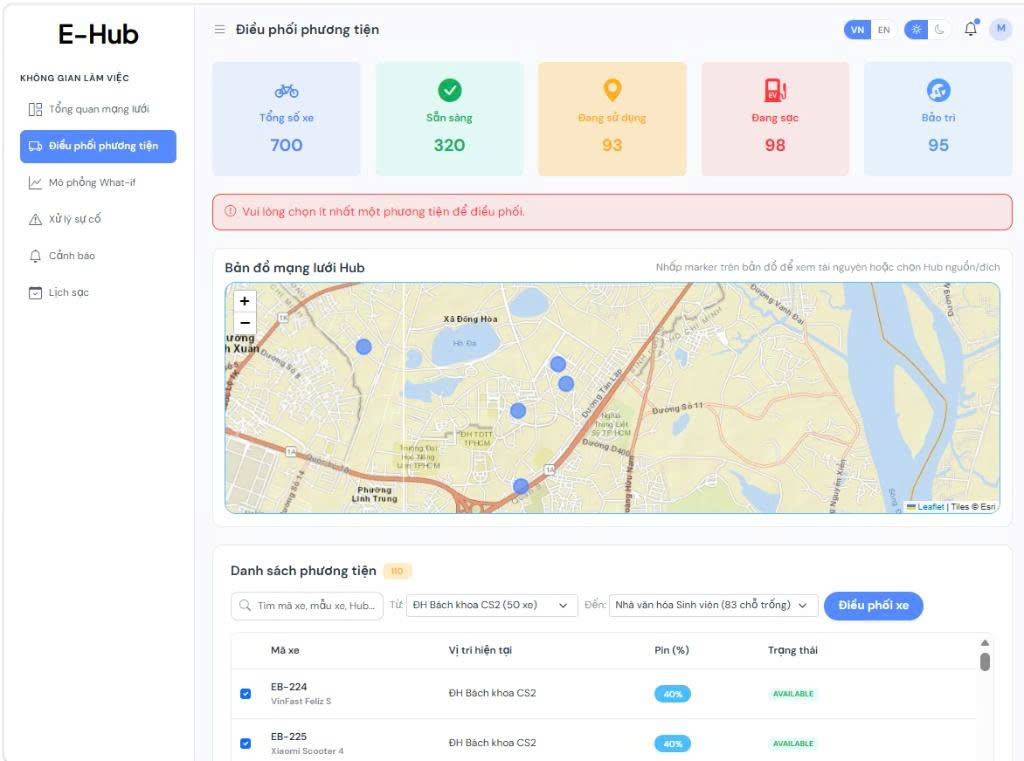
\includegraphics[width=\textwidth]{demo_UC1-17/UC11_dieu_phoi_phuong_tien_2_chon_xe.jpg}
        \caption{Chọn danh sách phương tiện cần điều phối}
    \end{subfigure}

    \vspace{0.3cm}
    \begin{subfigure}[b]{0.68\textwidth}
        \centering
        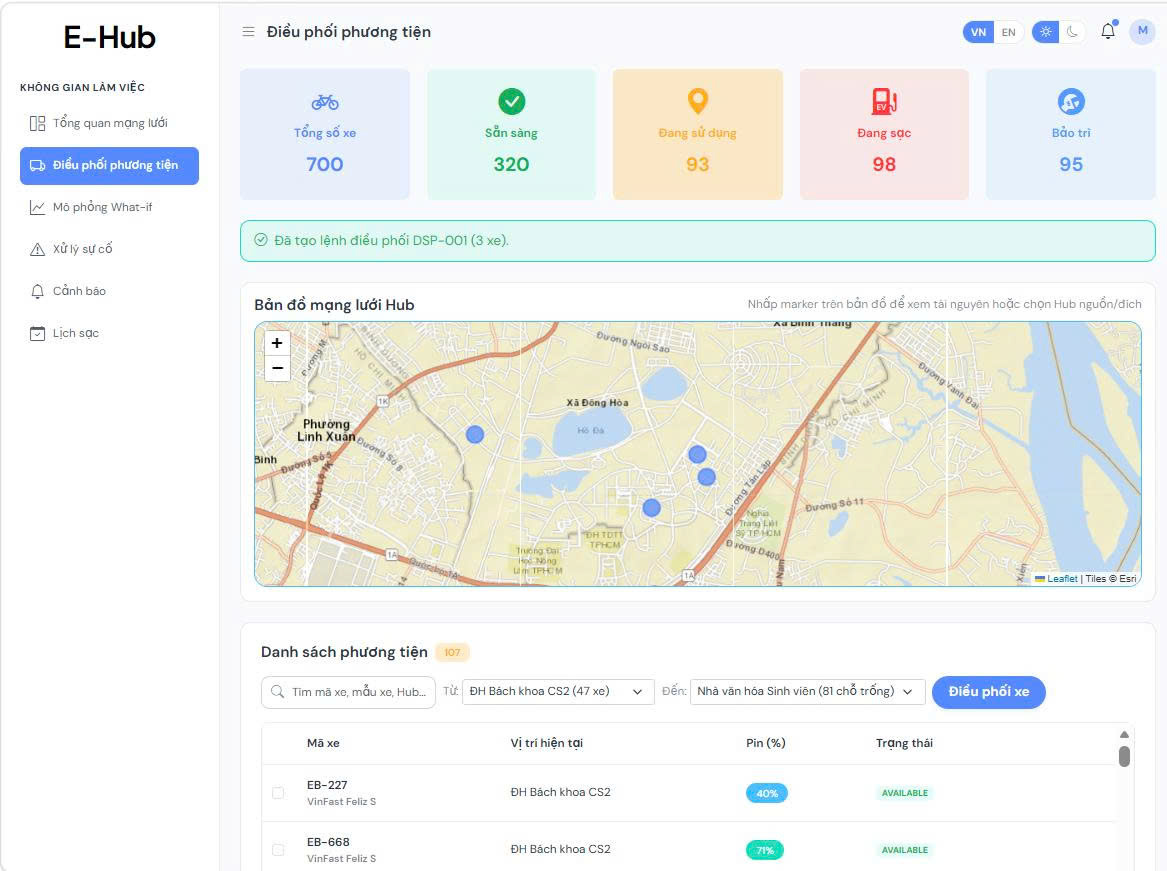
\includegraphics[width=\textwidth]{demo_UC1-17/UC11_dieu_phoi_phuong_tien_3_thanh_cong.jpg}
        \caption{Xác nhận tạo lệnh điều phối thành công}
    \end{subfigure}
    \caption{UC11 --- Quy trình điều phối phương tiện giữa các Hub}
    \label{fig:demo_uc11}
\end{figure}

\paragraph{UC12 --- Xử lý sự cố:}
Ghi nhận, theo dõi danh sách sự cố theo Hub/xe và cập nhật trạng thái xử lý trên màn hình chi tiết sự cố (\texttt{/operator/incidents}).
\begin{figure}[H]
    \centering
    \begin{subfigure}[b]{0.48\textwidth}
        \centering
        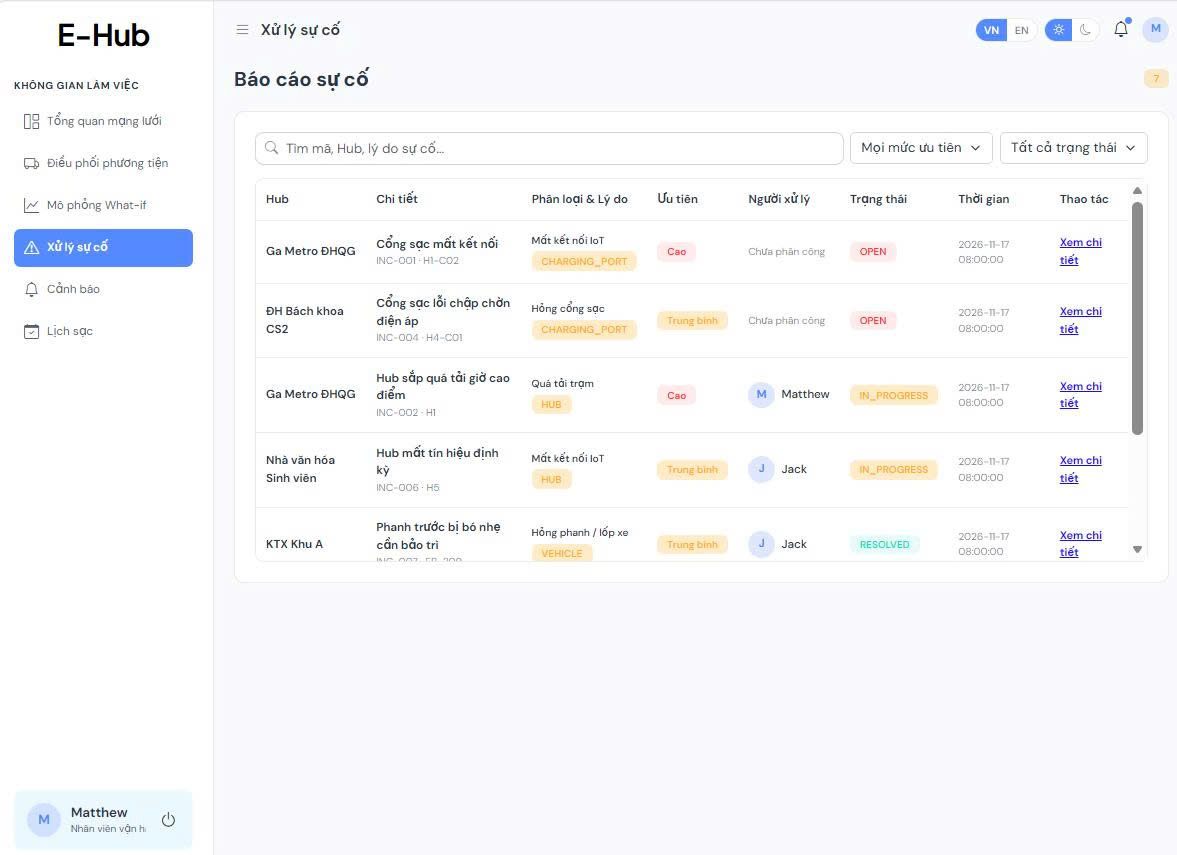
\includegraphics[width=\textwidth]{demo_UC1-17/UC12_xu_ly_su_co_1_danh_sach.jpg}
        \caption{Danh sách sự cố và biểu mẫu ghi nhận nhanh}
    \end{subfigure}
    \hfill
    \begin{subfigure}[b]{0.48\textwidth}
        \centering
        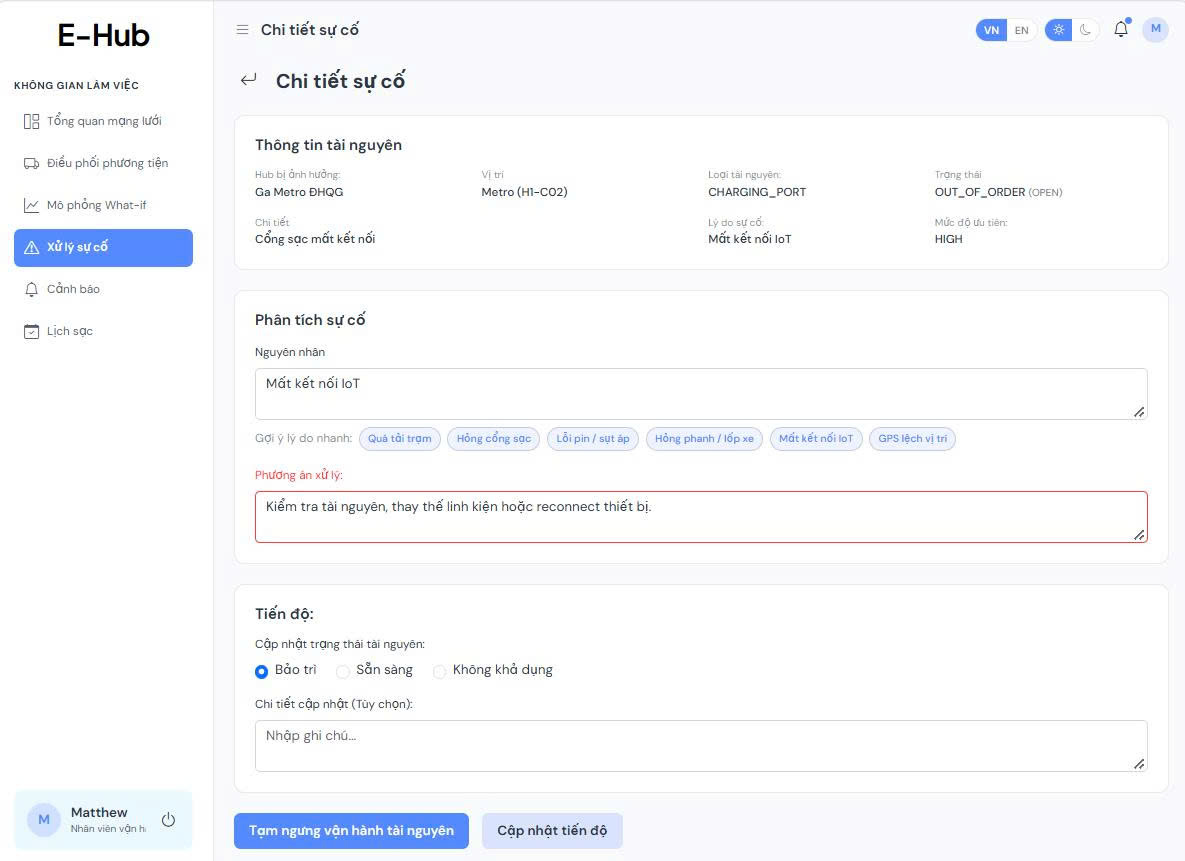
\includegraphics[width=\textwidth]{demo_UC1-17/UC12_xu_ly_su_co_2_chi_tiet.jpg}
        \caption{Chi tiết và thao tác xử lý sự cố}
    \end{subfigure}
    \caption{UC12 --- Quản lý và xử lý sự cố vận hành}
    \label{fig:demo_uc12}
\end{figure}

\paragraph{UC13 --- Lập lịch sạc thông minh:}
Hệ thống tự động đề xuất lịch sạc tối ưu cho các phương tiện pin yếu và cho phép Operator chỉnh sửa, phê duyệt (\texttt{/operator/schedule}).
\begin{figure}[H]
    \centering
    \begin{subfigure}[b]{0.48\textwidth}
        \centering
        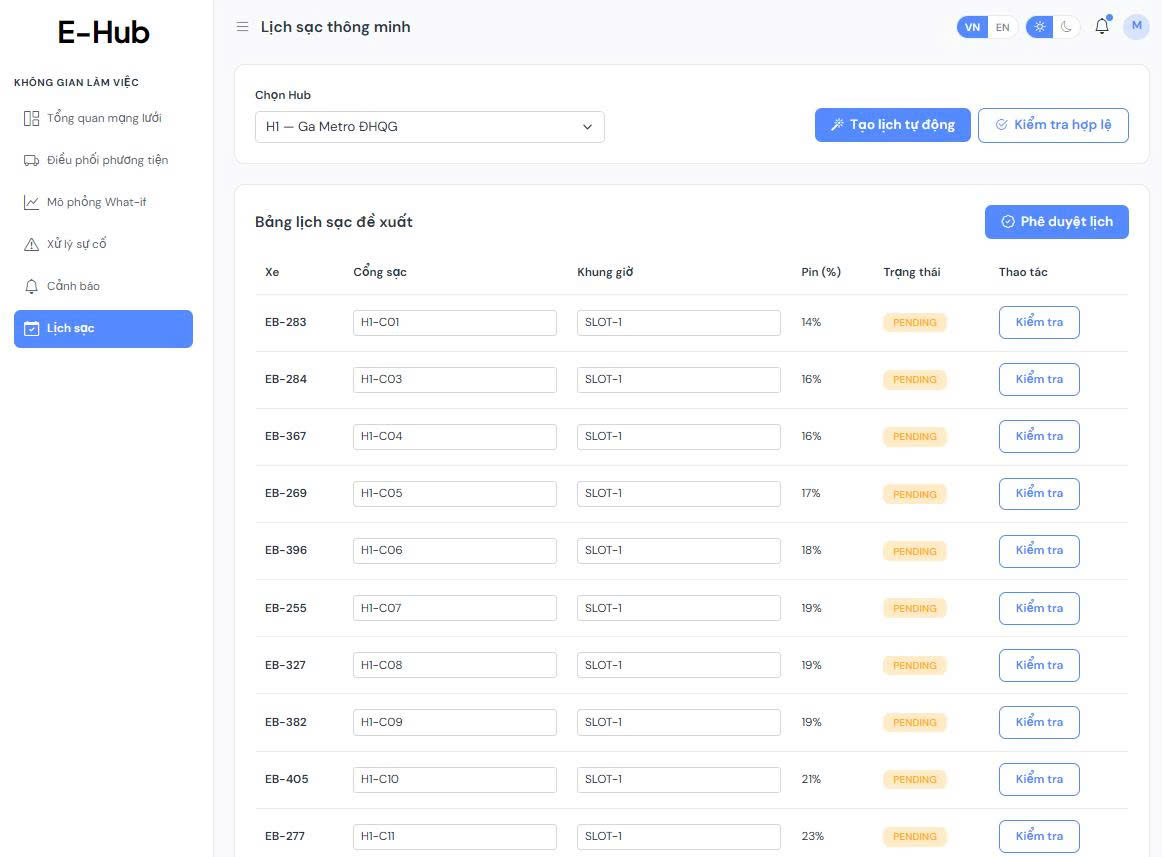
\includegraphics[width=\textwidth]{demo_UC1-17/UC13_lich_sac_thong_minh_1_de_xuat.jpg}
        \caption{Đề xuất lịch sạc theo Hub và mức pin}
    \end{subfigure}
    \hfill
    \begin{subfigure}[b]{0.48\textwidth}
        \centering
        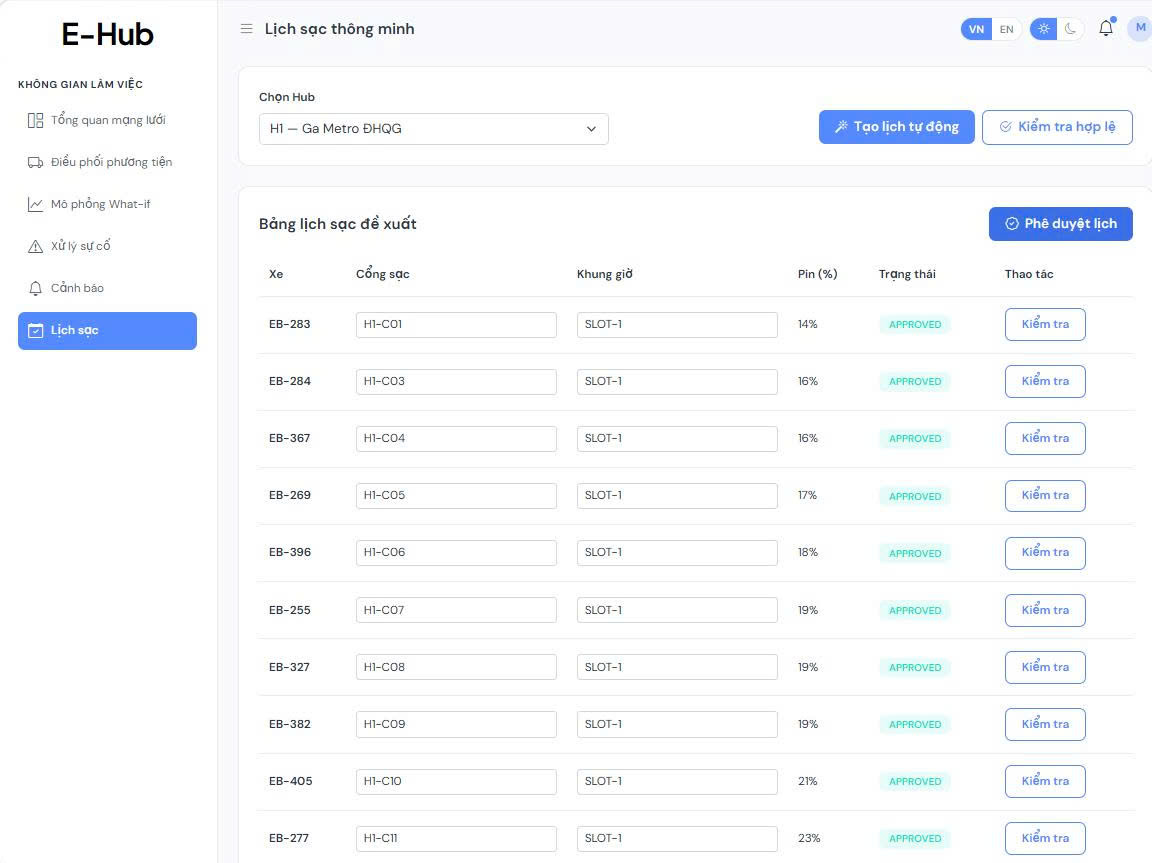
\includegraphics[width=\textwidth]{demo_UC1-17/UC13_lich_sac_thong_minh_2_phe_duyet.jpg}
        \caption{Phê duyệt lịch sạc thành công}
    \end{subfigure}
    \caption{UC13 --- Đề xuất và phê duyệt lịch sạc thông minh}
    \label{fig:demo_uc13}
\end{figure}

\paragraph{UC14 --- Mô phỏng What-if:}
Chạy thử kịch bản thời tiết, khung giờ và tình huống quá tải trên môi trường cô lập, xuất biểu đồ Chart.js và khuyến nghị điều phối mà không làm thay đổi dữ liệu vận hành thật (\texttt{/operator/simulation}).
\begin{figure}[H]
    \centering
    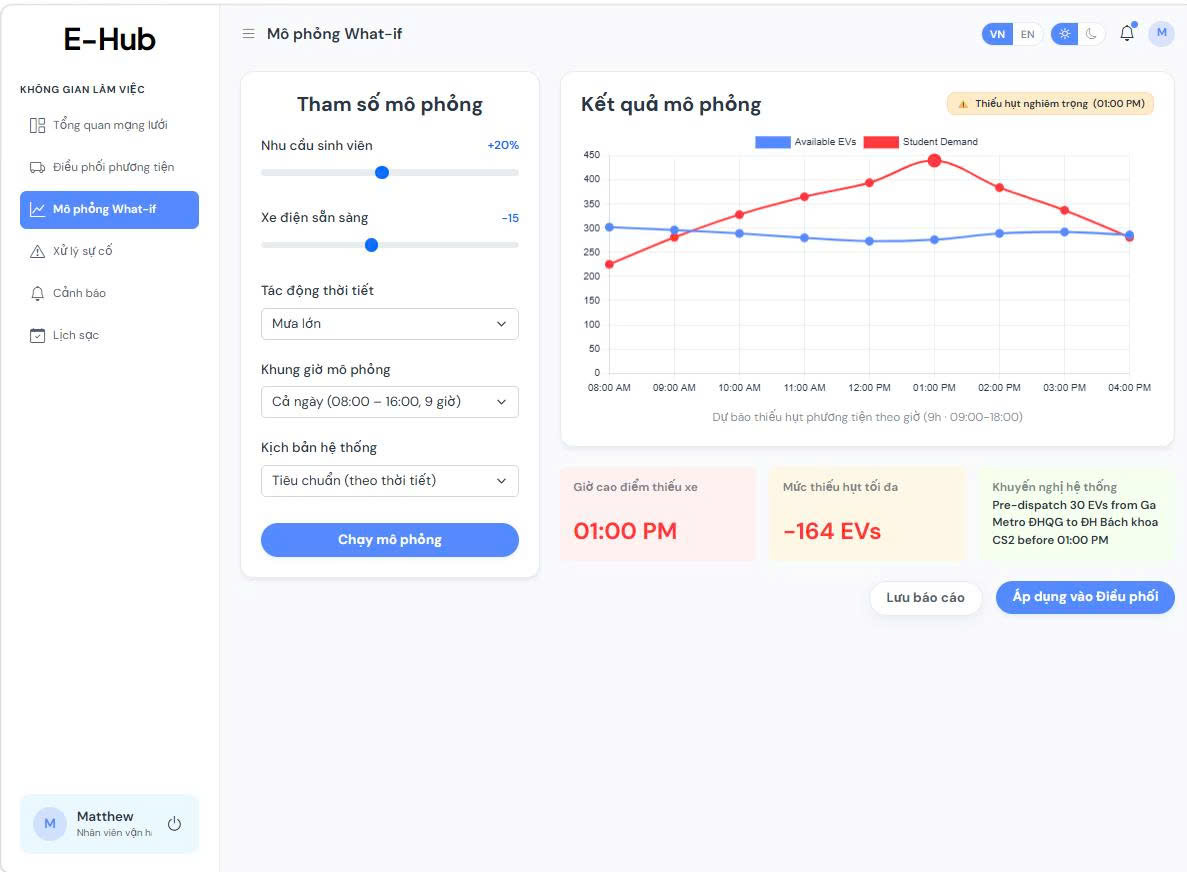
\includegraphics[width=0.88\textwidth]{demo_UC1-17/UC14_mo_phong_what_if.jpg}
    \caption{UC14 --- Kết quả mô phỏng What-if với biểu đồ nhu cầu và nguồn cung}
    \label{fig:demo_uc14}
\end{figure}

\paragraph{UC16 --- Cập nhật trạng thái \& Lọc gói trễ:}
Minh họa demo bắt buộc lọc và loại bỏ gói tin telemetry trễ (\texttt{scripts/packet\_demo.py}), ghi nhận trạng thái \texttt{ACCEPTED}/\texttt{OUTDATED\_IGNORED} vào bảng \texttt{PACKET\_LOG} trên Dashboard.
\begin{figure}[H]
    \centering
    \begin{subfigure}[b]{0.88\textwidth}
        \centering
        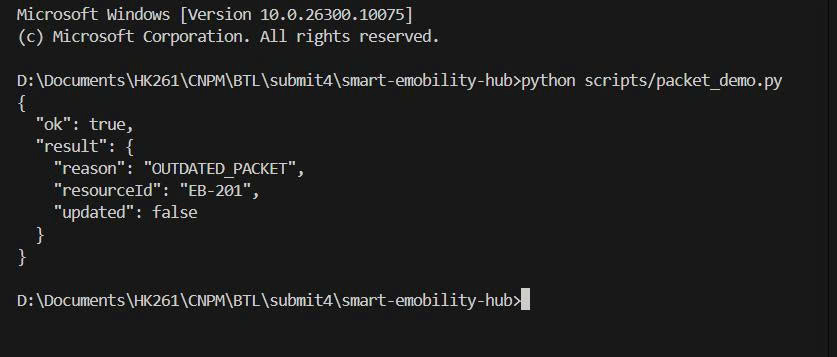
\includegraphics[width=\textwidth]{demo_UC1-17/UC16_cap_nhat_trang_thai_1_terminal.jpg}
        \caption{Kết quả chạy kịch bản demo lọc gói trễ (\texttt{scripts/packet\_demo.py})}
    \end{subfigure}

    \vspace{0.3cm}
    \begin{subfigure}[b]{0.88\textwidth}
        \centering
        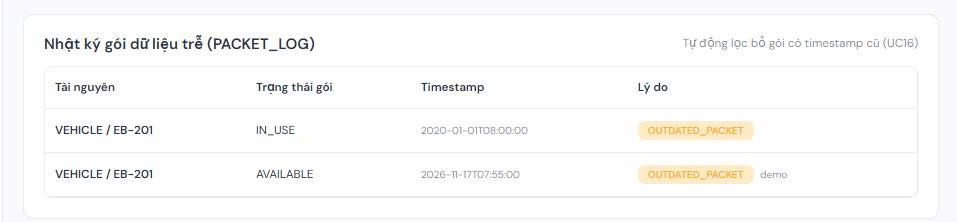
\includegraphics[width=\textwidth]{demo_UC1-17/UC16_cap_nhat_trang_thai_2_packet_log.jpg}
        \caption{Nhật ký gói tin \texttt{PACKET\_LOG} hiển thị trên trang tổng quan Operator}
    \end{subfigure}
    \caption{UC16 --- Cơ chế cập nhật trạng thái thời gian thực và lọc gói dữ liệu trễ}
    \label{fig:demo_uc16}
\end{figure}
